\section{Iterative center of mass displacement compensation algorithm}\label{sec:Algorithm}
In reality, the distribution of the center of mass within the body is not known, and therefore, an analytic solution provided with (\ref{eq:CMsolution2}) is impossible to calculate, thus an iterative method, based on repetitive hopping response is proposed. When a quadruped is continuosly jumping, its contact with the ground is infitesimally short, and consequently, reaction forces and torques can be approximated with the Dirac function $\delta (s)$. During the jump, the body behaves according to the Euler body dynamics function (\ref{eq:EulerBody}). Taking account the infitessimally short time the body has to accelerate (i.e. the rotation speeds are small, and their product is event smaller) the cross coupling term $\vec{\omega}\times J_B\vec{\omega}$ can be neglected and, consequently, the rotation speed vector can be approximated with (\ref{eq:RotSpeedAprox}).
\begin{figure}
	\centering
	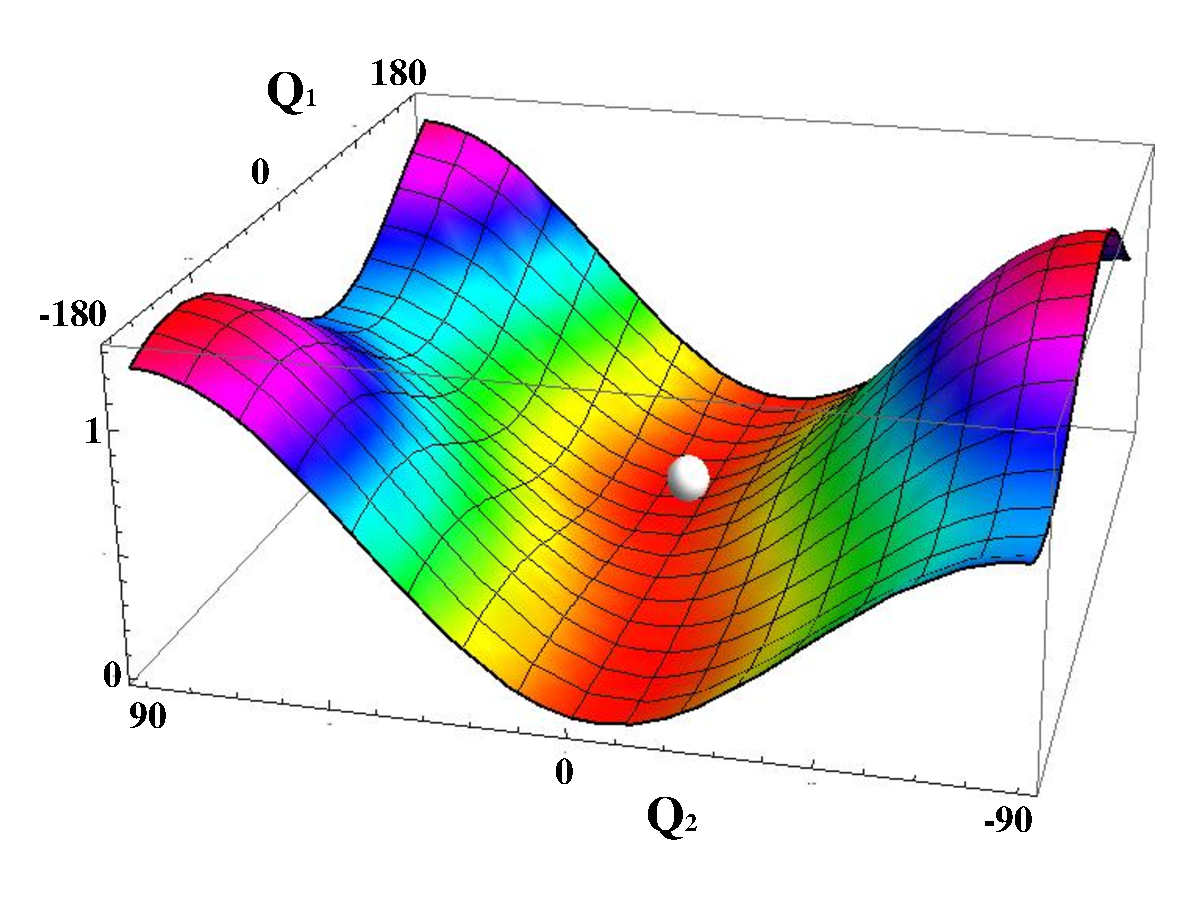
\includegraphics[width=85mm]{./pictures/RobinRepicCM.pdf}
	\caption{Center of mass displacement}
	\label{fig:CM3Dfunction}
\end{figure}

\begin{equation}\label{eq:EulerBody}
\tau_{tot}=J_B\vec{\dot{\omega}}+\vec{\omega}\times J_B\vec{\omega}
\end{equation}

\begin{equation}\label{eq:RotSpeedAprox}
\vec{\omega}\approx \frac{1}{s}{J_B}^{-1}\begin{bmatrix}
\Delta \textsc{cm}_y & -\Delta \textsc{cm}_x & 0
\end{bmatrix}^T\bar{T}\delta(s)
\end{equation}

Calculating the absolute value of vector (\ref{eq:RotSpeedAprox}) it is easy to show that the size of the rotation speed vector is proportional to the displacement of center of mass \eqref{eq:WpropCM}. In other words, centering the robot and minimizing the displacement of the center of mass eliminates the generation of unwanted rotations. 

\begin{equation}\label{eq:WpropCM}
\left \| \vec{\omega} \right \|\sim \sqrt{{\Delta \textsc{cm}_x}^2+{\Delta \textsc{cm}_y}^2}
\end{equation}


In order to iteratively calculate the angles $q1$ and $q2$, angular velocity vector is recorded during start of hopping acceleration phase $F_1$. This phase lasts until one of the leg/spring reaches desired length $L_d$. The leg which carries a minimum mass will achieve the fastest acceleration and the algorithm task is to navigate tail towards this leg. 

For example, mass distribution in figure  (\ref{fig:imassCom}) is equally distributed except for $MASS_2$  which is lighter then others. At the end of phase $F_1$ the body rotates at an angular velocity $\vec{\omega}$. By using the cross product of projection vector $\vec{\omega_{xy}}$ in $XY$ plane and body $\vec{Zb}$, the tail direction vector $\vec{\omega_{TD}}$ is calculated. 

Tail motion control algorithm navigates tail in vector $\vec{\omega_{TD}}$ direction which at the end results the equal mass distribution.

\begin{algorithm}
\caption{Minimize $\left \| \vec{\omega} \right \|\sim \sqrt{{\Delta \textsc{cm}_x}^2+{\Delta \textsc{cm}_y}^2}$}
\begin{algorithmic} 
\STATE $y \leftarrow 1$
\REPEAT
\STATE $Q_1 = $
\STATE $Q_2 = $
\REPEAT
\STATE JUMP
\STATE $W = \int \left \| \vec{\omega}(t) \right \|  dt$
\STATE $Dir = atan2(\omega_y,\omega_x)$
\UNTIL JUMP COMPLETE
\STATE Calculate new $Q_1$ and $Q_2$
\UNTIL{$W < $ limit}
\end{algorithmic}
\end{algorithm}


\begin{figure}
	\centering
	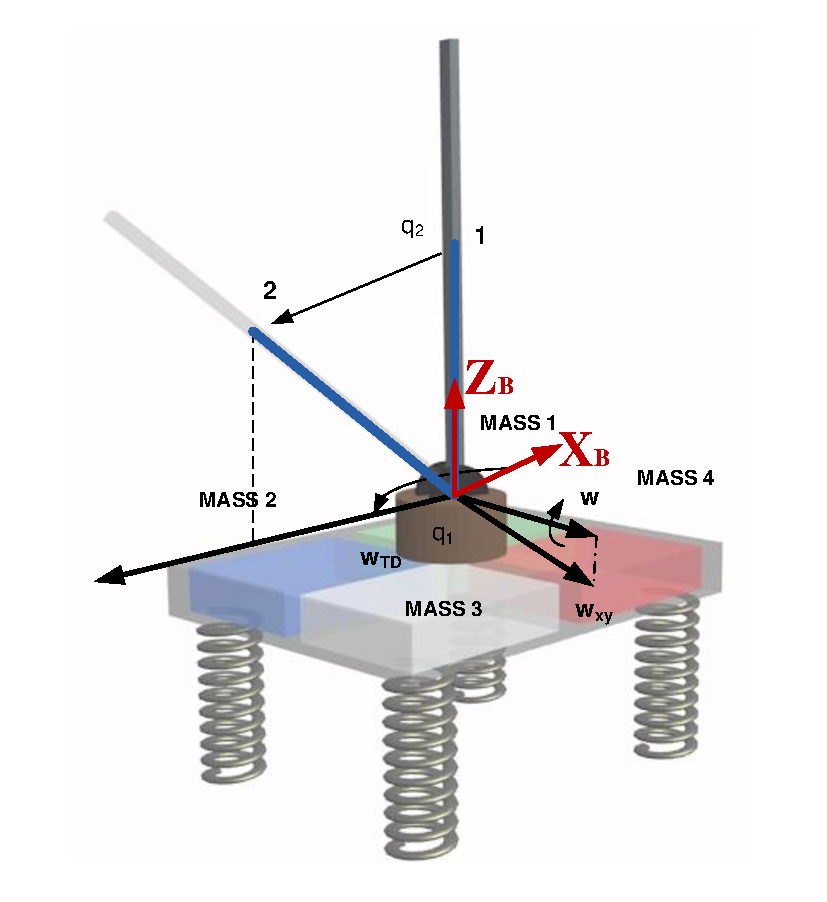
\includegraphics[width=85mm]{./pictures/IterativeAlgorithm.pdf}
	\caption{Iterative mass displacement compensation}
	\label{fig:imassCom}
\end{figure}